\documentclass{beamer}
\usepackage[utf8]{inputenc}
\usepackage{xcolor}
\usepackage{algorithm}
\usepackage{algorithmic}
\usepackage[T1]{fontenc}
\usepackage[normalem]{ulem}
\usetheme{Antibes}

\title{Optimization Project:\\Support Vector Machine}
\author{K. Kamtue \& Cl. Réda}
\institute{\textsc{ENS Cachan}}
\date{January 12th, 2017}

\setbeamerfont{page number in head/foot}{size=\large}
\setbeamertemplate{footline}[frame number]

\begin{document}
\maketitle
\tableofcontents
\setlength{\parindent}{1cm}

\section{Project description}

\subsection{Project}

\begin{frame}
\tableofcontents[currentsubsection]
\end{frame}

\begin{frame}
\frametitle{Project}
\framesubtitle{\textbf{Support Machine Vector}}

\begin{alertblock}{Objective}
\begin{center}
\textbf{Classify} data
\end{center}
\end{alertblock}

\pause

\begin{itemize}
\item Applied to \textbf{binary classification} ($y_i \in \{1, -1\}$);

\pause

\item Looking for a \textbf{hyperplane} $f : x \rightarrow \omega^Tx$ $(+ b)$ such as:
         
          \begin{center}
           \begin{equation}
         \forall i, f(x_i) = 
         \begin{cases}
         <0 &\mbox {si y=-1} \\
         >0 &\mbox {si y=1}
         \end{cases}
         \Leftrightarrow \forall i, y_i \times f(x_i) > 0 
         \end{equation}
         \end{center}
\end{itemize}

\end{frame}

\begin{frame}
\frametitle{Project}
\framesubtitle{\textbf{Support Machine Vector}}

         \begin{figure}
         \centering
         \caption{Example with two classes (\textbf{red} and \textbf{blue})}
         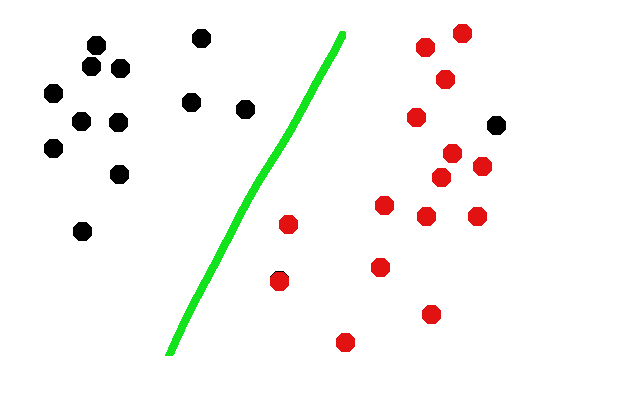
\includegraphics[scale=0.4]{images/voronoi.png}
         \end{figure}

\end{frame}

\subsection{Optimization problem}

\begin{frame}
\frametitle{Optimization problem}
\framesubtitle{Looking for the optimization problem}

\begin{block}{Naive optimization problem}
$\gamma$: distance between the lines $f(x) = 1$ and $f(x) = -1$.

\pause

      \begin{center}
        $max_{\omega}$ $\gamma = \frac{2}{\|\omega\|}$\\
        subject to $\forall i, y_i \times f(x_i) > 0$\\

\pause

       \bigskip
        $\Leftrightarrow min_{\omega}$ $\frac{1}{2} \|\omega\|^2$\\
        subject to $\forall i, y_i \times f(x_i) > 0$\\
      \end{center}

\end{block}

\textbf{Beware:} if the data set is not linearly \underline{separable}!

\end{frame}

\begin{frame}
\frametitle{Optimization}
\framesubtitle{Looking for the optimization problem}

         \begin{figure}
         \centering
         \caption{Example with two classes (\textbf{red} and \textbf{blue})}
         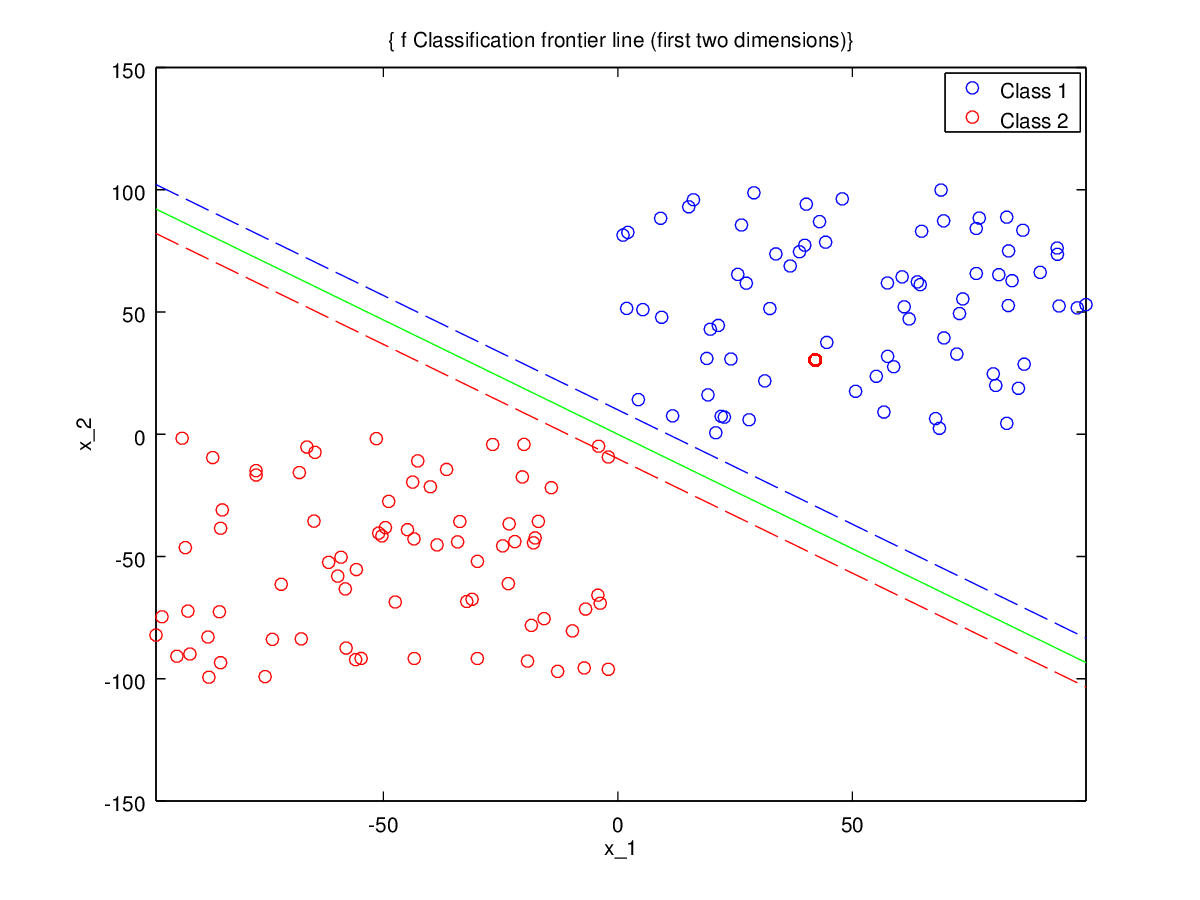
\includegraphics[scale=0.4]{images/voronoi2.png}
         \end{figure}

\end{frame}

\begin{frame}
\frametitle{Optimization problem}
\framesubtitle{Adapting the problem to \textbf{non-separable sets}}

Let $z_i$ be $max(0, 1-y_i \times f(x_i))$ (\textbf{Hinge loss}).

\pause

\bigskip

\begin{block}{Having the problem \textbf{convex} and always \textbf{feasible}}

Penalty for \textbf{classification errors} with $(z_i)_i$ and $C$ :

           \begin{center}
           $min_{\omega, z}$ $\frac{1}{2} \|\omega\|^2 + C \sum_{i \leq m}z_i$\\
           subject to\\ $\forall i, z_i \geq 0$\\
           $\forall i, y_i \times (\omega^{T} x_i) \geq 1 - z_i$\\
           \end{center}

\end{block}

\end{frame}

\subsection{Implementation}

\begin{frame}
\tableofcontents[currentsubsection]
\end{frame}

\begin{frame}
\frametitle{Implementation}
\framesubtitle{Solving the optimization problem}

\begin{itemize}
\item Use \textbf{Newton's method}:

\bigskip

\begin{block}{\underline{Reminder}: Update of $x$ with \textbf{Newton's method}}
          \begin{center}
          $x_{n+1} \leftarrow x_{n} + s \times \nabla^2 obj(x_n)^{-1}\nabla obj(x_n)$
          \end{center}

  (finding \textbf{step size} value $s$ by \textbf{backtracking line search})
\end{block}

\bigskip
\pause

\item Make the problem independant from \textbf{dimension};

\bigskip
\pause

\item Use \textbf{logarithmic barrier method}.

\end{itemize}

\end{frame}

\begin{frame}
\frametitle{Implementation}
\framesubtitle{Independance from dimension: \textbf{dual problem}}

After Lagrangian calculation and minimization in $\omega$: 

\bigskip
\pause

\begin{block}{\textbf{Dual problem}}
             \begin{center}
             $max_{\lambda \in \mathbb{R}^{+m}} -\frac{1}{2}\|\sum_i\lambda_iy_ix_i\|^2_2 + $\textbf{1}$^T\lambda$\\ 
             subject to $\forall i, 0 \leq \lambda_i \leq C$\\
          
             (\textbf{KKT conditions})
             \end{center}
\end{block}

\pause

\begin{alertblock}{Get \textbf{primal solution} from \textbf{dual solution}}
             \begin{center}
               $\omega^{*} = \sum_i \lambda^{*}_i y_i x_i$
             \end{center}
\end{alertblock}

\end{frame}

\begin{frame}
\frametitle{Implementation}
\framesubtitle{Make the problem independant from dimension}

Use the \textbf{kernel trick} :

\bigskip

\begin{block}{\textbf{Dual problem}}
Let $K$ be $X^TX$ (\textbf{linear kernel}):

\bigskip
                 \begin{center}
                 $max$ $-\frac{1}{2}\lambda^Tdiag(y)Kdiag(y)\lambda+$\textbf{1}$^T\lambda$\\
                 subject to $\forall i, 0 \leq \lambda_i \leq C$ 
                 \end{center}
\end{block}

\end{frame}

\begin{frame}
\frametitle{Implementation}
\framesubtitle{Delete inequality constraints}

Use the \textbf{logarithmic barrier method} :

\pause

\begin{block}{Barrier function}
          \begin{center}
          $\Phi(\lambda) = \sum_i (- log(C - \lambda_i) - log(\lambda_i))$\\
          $= - \sum_i log((C - \lambda_i)\lambda_i)$ 
          \end{center}
\end{block}

\pause

\begin{alertblock}{Final optimization problem}
          \begin{center}
          $max$ $-\frac{1}{2}\lambda^Tdiag(y)Kdiag(y)\lambda+$\textbf{1}$^T\lambda + \Phi(\lambda)$\\ 
          \end{center}
\end{alertblock}

\end{frame}

\section{Results}

\subsection{Testing the implementation}

\begin{frame}
\tableofcontents[currentsubsection]
\end{frame}

\begin{frame}
\frametitle{Testing the implementation}
\framesubtitle{\textbf{Newton's method} convergence}


         \begin{figure}
         \centering
         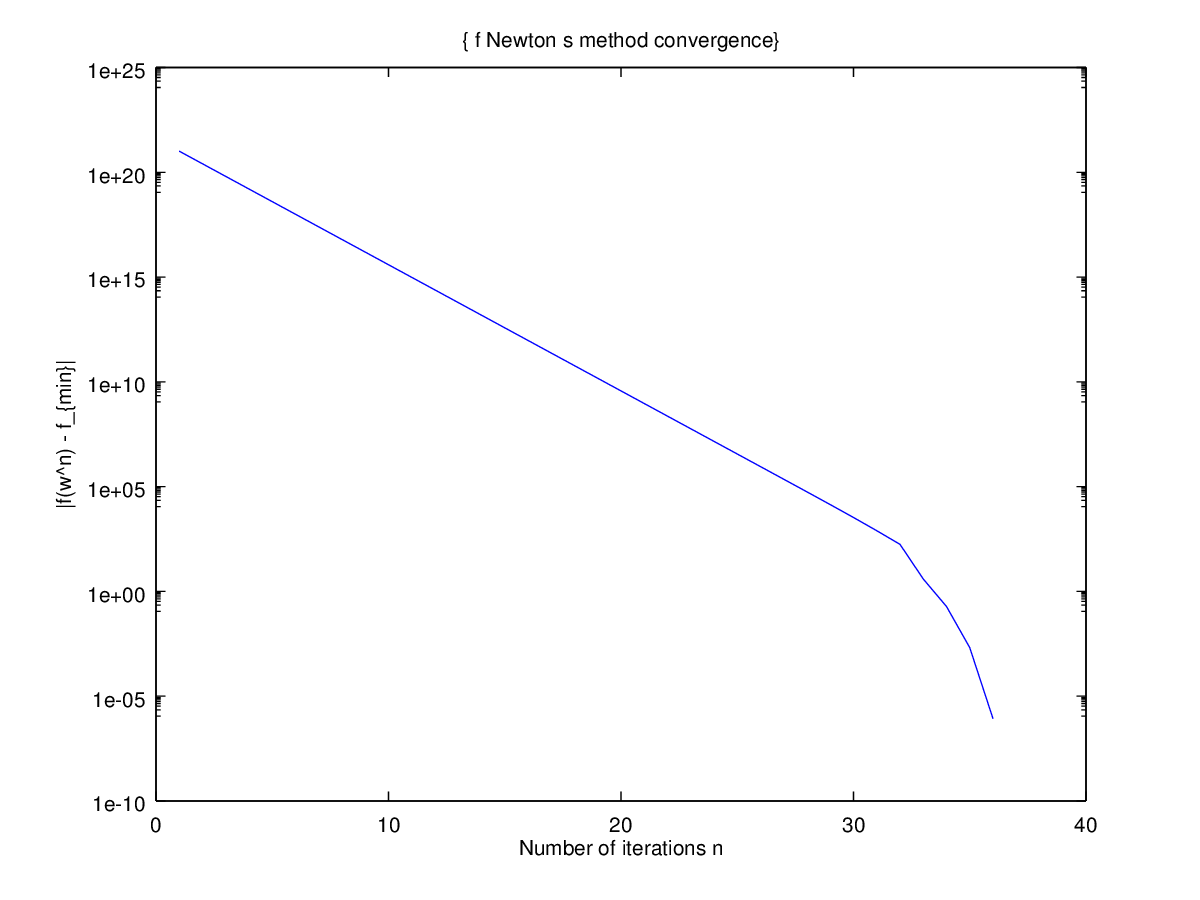
\includegraphics[scale=0.4]{images/cvnewton4.png}
         \end{figure}

\end{frame}

\begin{frame}
\frametitle{Testing the implementation}
\framesubtitle{Dependance on the sample size}

                \begin{table}
                \centering
                \caption{Time complexity dependance}
                \begin{tabular}{| l | c | c | c | c | r |}
                \hline
                Set & C & d & n & Iteration number & Time (s) \\ \hline
                1 & 5 & 40000 & 10 & 11 & 0.315 \\ \hline
                1 & 5 & 40 & 100 & 12 & 0.715 \\ \hline
                1 & 5 & 40 & 1000 & large & > 1,000 \\ \hline
                \end{tabular}
                \end{table}

\end{frame}

\begin{frame}
\frametitle{Testing the implementation}
\framesubtitle{Performance in function of $C$}

Performed on the same sample set:\\

                \begin{table}
                \centering
                \caption{Computation time \& Performance in function of C}
                \begin{tabular}{| l | c | c | c | r |}
                \hline
               C  & Time (s) & Training Error & Val Error & Test Error\\ \hline
               1 & 132.15 & 6 & 2 & 3\\ \hline
               10  & 0.74 & 6 & 2 & 3\\ \hline
               100  & 0.89 & 1 & 12 & 3\\ \hline
                \end{tabular}
                \end{table}

\end{frame}

\subsection{Plotting the classification frontier}

\begin{frame}
\tableofcontents[currentsubsection]
\end{frame}

\begin{frame}
\frametitle{Plotting the \textbf{classification frontier}}
\framesubtitle{For $C = 5, n = 150, d = 200$}

Normalized points with Gaussian distribution (2D):

         \begin{figure}
         \centering
         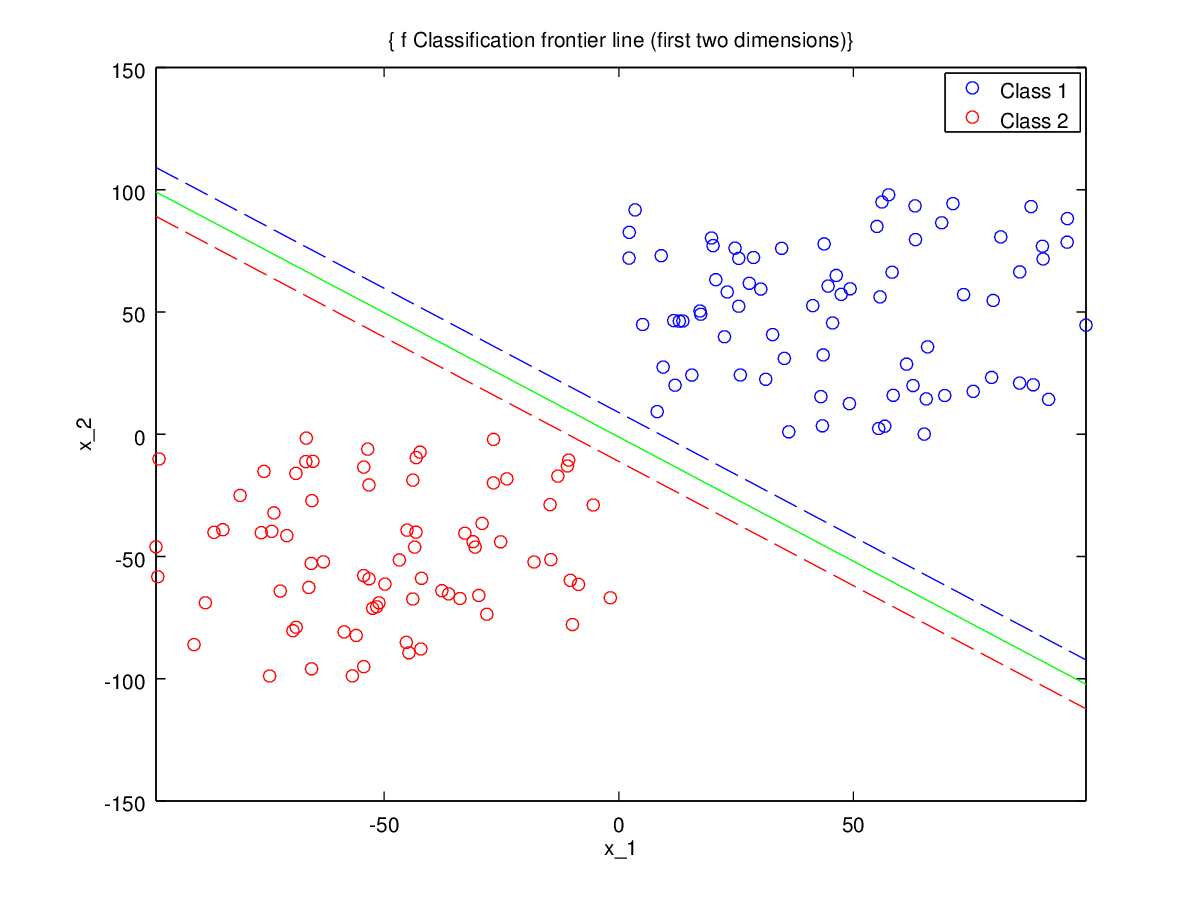
\includegraphics[scale=0.4]{images/line4.png}
         \end{figure}

\end{frame}

\begin{frame}
\frametitle{Plotting the \textbf{classification frontier}}
\framesubtitle{For $C = 5, n = 150, d = 200$}

Normalized points with Gaussian distribution (3D):

         \begin{figure}
         \centering
         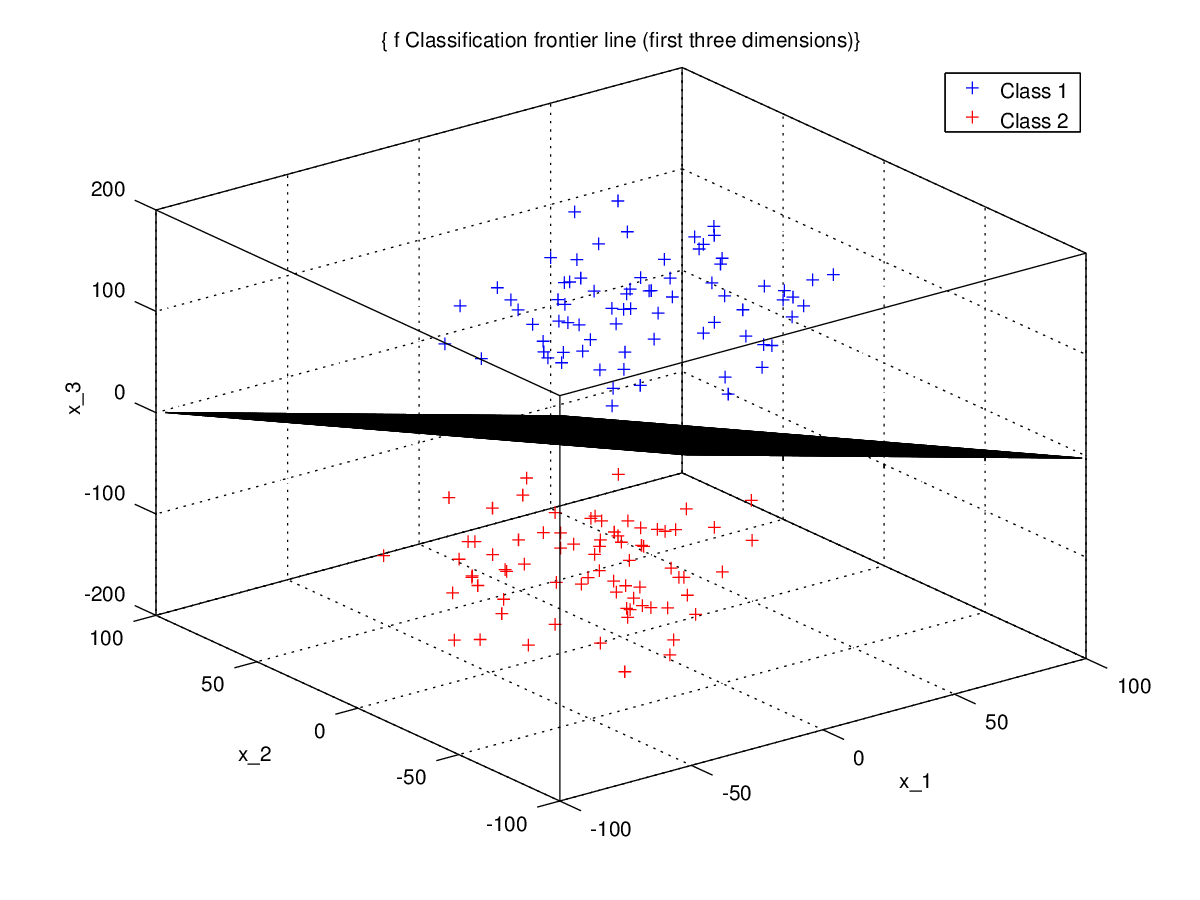
\includegraphics[scale=0.4]{images/plane4.png}
         \end{figure}

\end{frame}

\begin{frame}
\frametitle{Plotting the \textbf{classification frontier}}
\framesubtitle{Pour $C = 5, n = 100, d = 2$}

Generation with Gaussian distribution (2D) (set A) :

         \begin{figure}
         \centering
         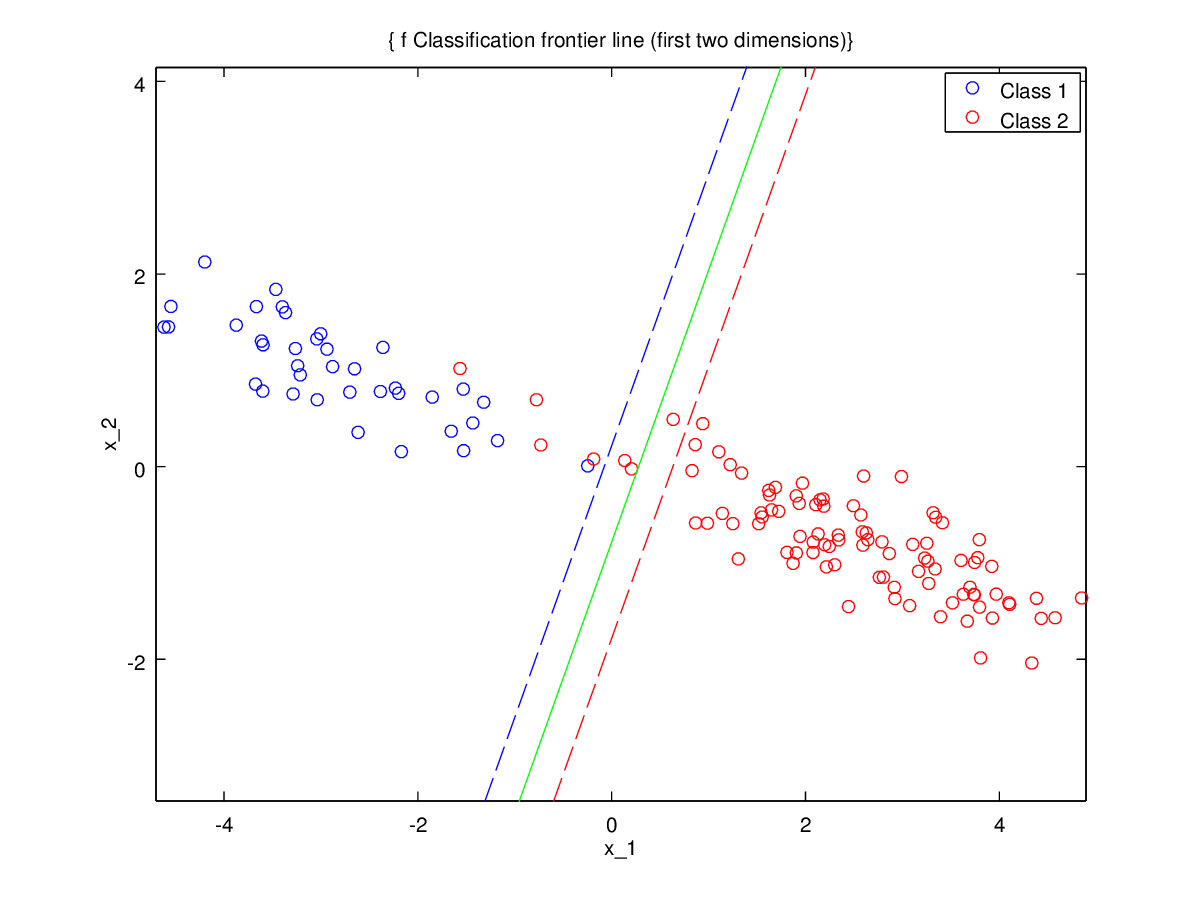
\includegraphics[scale=0.4]{images/image1.png}
         \end{figure}

\end{frame}

\begin{frame}
\frametitle{Plotting the \textbf{classification frontier}}
\framesubtitle{Pour $C = 5, n = 100, d = 2$}

Generation with Gaussian distribution (2D) (set B) :

         \begin{figure}
         \centering
         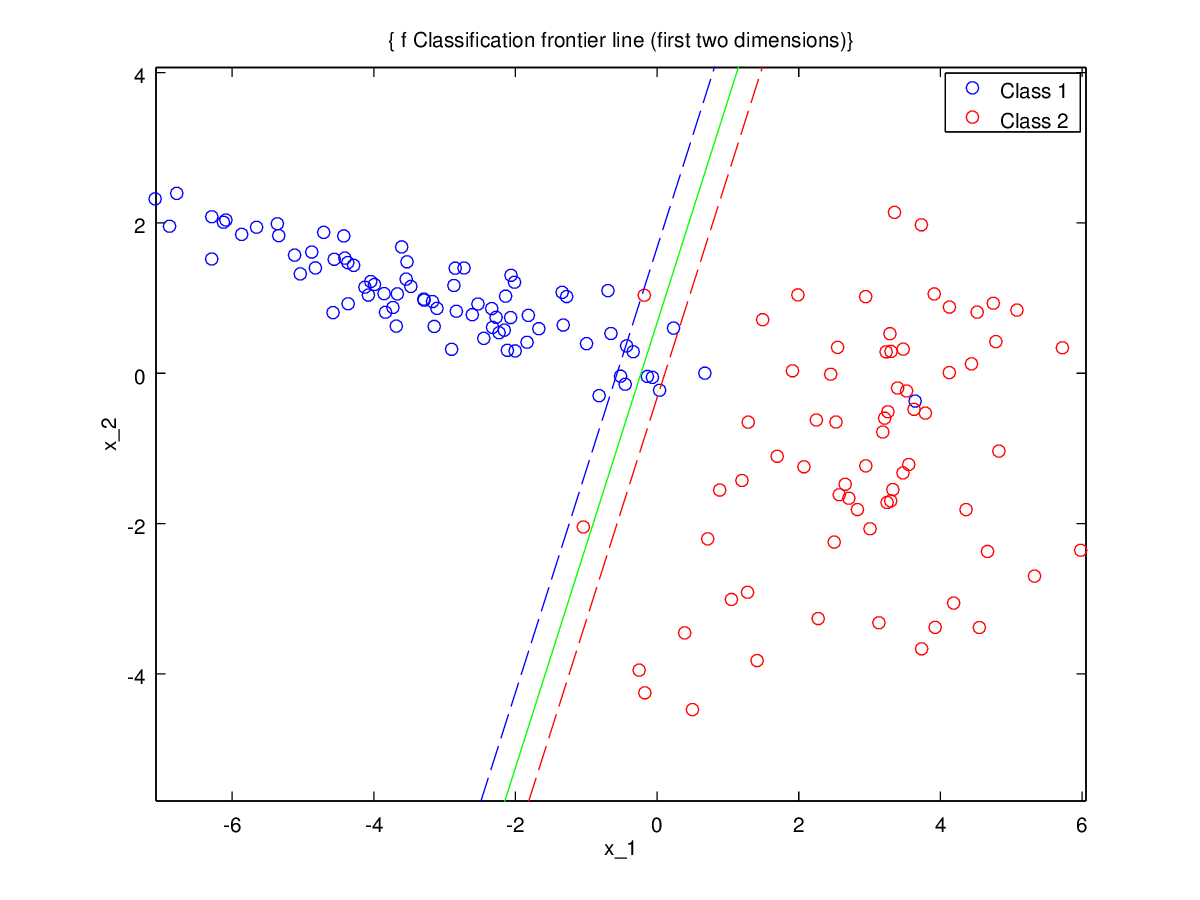
\includegraphics[scale=0.4]{images/image2.png}
         \end{figure}

\end{frame}

\section{Extensions}

\subsection{Cross Validation}

\begin{frame}
\tableofcontents[currentsubsection]
\end{frame}

\begin{frame}
\frametitle{Extensions}
\framesubtitle{Cross Validation}

\begin{itemize}
\item \textbf{Cross validation} (choice of the best value for C);
\end{itemize}

\bigskip
\pause

\begin{block}{Leave-one-out technique}
\textbf{Having a sample size of size $n$}, for each value of C to test:\\
\begin{enumerate}
\item for $i \in [1, n]$
\item \textbf{Leave out sample} $i$
\item Train the SVM on other samples 
\item Test the SVM on sample $i$
\item Get the \textbf{Mean-Squared Error} for the $n$ loops
\item If it is the minimum MSE computed so far
\item Then update the best value of C
\end{enumerate}
\end{block}

\end{frame}

\subsection{Coordinate Descent}

\begin{frame}
\tableofcontents[currentsubsection]
\end{frame}

\begin{frame}
\frametitle{Extensions}
\framesubtitle{Coordinate Descent}

\begin{itemize}

\item Implementation of \textbf{Coordinate Descent};

\bigskip
\pause

\end{itemize}

\begin{block}{\underline{Reminder:} Coordinate Descent}
for $i, j \in [1, d]$, and iteration $k$\\
\begin{center}
$a_i^{k+1} = argmin_{a_i} f(a_1, a_2, ..., a_i, ..., a_d)$\\
$a_j^{k+1} = a_j^{k}$ for $j \neq i$
\end{center}
\end{block}

\end{frame}

\begin{frame}
\frametitle{Extensions}
\framesubtitle{Coordinate Descent results}

Performed on the same sample set (as in the testing of the original SVM):\\

                \begin{table}
                \centering
                \caption{Computation time \& Performance in function of C}
                \begin{tabular}{| l | c | c | c | r |}
                \hline
               C  & Time (s) & Training Error & Val Error & Test Error\\ \hline
               1 & 0.37 & 11 & 6 & 5.33\\ \hline
               10  & 0.34 & 5 & 4 & 3.39\\ \hline
               100  & 0.29 & 1 & 8 & 3.56 \\ \hline
               10,000 & 0.29 & 6 & 4 & 2.76\\ \hline
                \end{tabular}
                \end{table}

\end{frame}

\subsection{ACCPM}

\begin{frame}
\tableofcontents[currentsubsection]
\end{frame}

\begin{frame}
\frametitle{Extensions}
\framesubtitle{ACCPM}

\begin{itemize}

\item Implementation of \textbf{Analytic Center Cutting-Plane Method};

\bigskip
\pause

\begin{block}{\underline{Reminder:} ACCPM}
\begin{enumerate}
\item Compute the \textbf{analytic center of constraint polyhedron} 
\item Compute the objective value and the gradient 
\item While objective value is evolving greatly enough
\item Add an inequality to constraint polyhedron 
\item \underline{Optional:} \textbf{Constraint Dropping}
\end{enumerate}
\end{block}

\end{itemize}

\end{frame}

\begin{frame}
\frametitle{Extensions}
\framesubtitle{ACCPM results}

\begin{figure}
\caption{For data of size 8, and dimension 2}
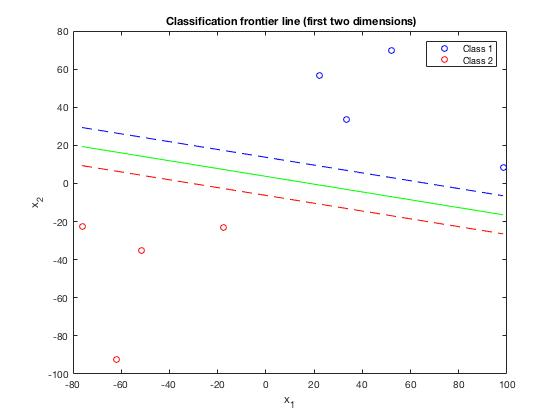
\includegraphics[scale=0.4]{images/accpmtestfig.jpg}
\end{figure}

\end{frame}

\section{Demo}

\begin{frame}
\tableofcontents[currentsection]
\end{frame}

\begin{frame}

\bigskip

\bigskip

\begin{center}
\textbf{Demo of the SVM}
\end{center}

\end{frame}


\end{document}